%
% Modelo de artigo científico em português brasileiro e em conformidade com as normas da ABNT
% Documento principal
%
% *****************************************************************************
% *  Centro Federal de Educação Tecnológica de Minas Gerais - CEFET-MG        *
% *  Laboratório de Sistemas Inteligentes - LSI                               *
% *                                                                           *
% *  Autor: Denise de Souza <densouza@gmail.com>                              *
% *  Autor: Henrique E. Borges <henrique@lsi.cefetmg.br>                      *
% *                                                                           *
% *****************************************************************************



\documentclass[
%   opções da classe memoir
      article,					% Indica que é um artigo científico
      %11pt,					% Tamanho da fonte
      twocolumn,				% Número de colunas
      %twoside,					% Impressão em frente (anverso) e verso. Oposto a oneside
      %oneside,					% Impressão apenas no anverso. Oposto a twoside
      a4paper,					% Tamanho do papel
%   opções da classe abntex2
      %chapter=TITLE,			% Títulos de capítulos convertidos para letras maiúsculas
      %section=TITLE,			% Títulos de seções convertidos para letras maiúsculas
      %subsection=TITLE,		% Títulos de subseções convertidos para letras maiúsculas
      %subsubsection=TITLE 		% Títulos de subsubseções convertidos para letras maiúsculas
%   opções do pacote babel
      english,					% Idioma adicional para hifenização
      brazil,					% O ultimo idioma indicado será o principal idioma do documento
      sumario=tradicional
]{abntex2} 



% -----------------------------------------------------------------------------
%    Pacotes fundamentais 
% -----------------------------------------------------------------------------

\usepackage[T1]{fontenc}		% Seleção de código de fonte
\usepackage{lmodern}			% Usa a fonte Latin Modern
%\usepackage[latin1]{inputenc}	% Codificação do documento (conversão automatica dos acentos)
\usepackage[utf8]{inputenc}		% Codificação do documento (conversão automatica dos acentos)
\usepackage{indentfirst}		% Indenta o primeiro parágrafo de cada seção.
\usepackage{nomencl} 			% Lista de símbolos
\usepackage{color}				% Controle das cores
\usepackage{graphicx}			% Inclusão de gráficos
\usepackage{microtype} 			% Melhora a justificação do documento
\usepackage{comandos} 			% Novos comandos
\usepackage{tikz}	 			% Pacote para desenhos
\usepackage{etoolbox}	 		% Pacote para tratamento de condicionais (if-else-end \ string)
\usepackage{ifthen}				% Pacote para tratamento de condicionais (if-else-end \ number)
\usepackage{balance}			% Balanceia o texto no artigo
\usepackage{babel}				% Usado para definir idioma do documento e respectivas hifenizações



% -----------------------------------------------------------------------------
%    Configura as citações
% -----------------------------------------------------------------------------

\usepackage[alf]{abntex2cite}		% Formata as citações bibliográficas conforme a norma ABNT
%\usepackage[alf, 					% Formata as citações bibliográficas conforme a norma ABNT
%	abnt-emphasize=bf, 
%	bibjustif, 
%	recuo=0cm, 
%	abnt-etal-cite=2, 
%	abnt-etal-list=0]{abntex2cite}


% -----------------------------------------------------------------------------
%   Configurações de aparência do PDF final
% -----------------------------------------------------------------------------

\definecolor{blue}{RGB}{41,5,195}	% Altera o aspecto da cor azul

\makeatletter
\hypersetup{
  %pagebackref=true,
  %pdftitle={\@title}, 
  %pdfauthor={\@author},
  %pdfsubject={Modelo de artigo científico com abnTeX2},
  %pdfcreator={LaTeX with abnTeX2},
  %pdfkeywords={abnt}{latex}{abntex}{abntex2}{artigo científico}, 
  colorlinks=true,       	% true: “links” coloridos; false: “links” em caixas de texto
  linkcolor=blue,			% Define cor dos “links” internos”
  citecolor=blue,			% Define cor dos “links” para as referências bibliográficas
  filecolor=magenta,		% Define cor dos “links” para arquivos
  urlcolor=blue,			% Define a cor dos “hiperlinks”
  bookmarksdepth=4
}
\makeatother



% -----------------------------------------------------------------------------
%   Compila o índice
% -----------------------------------------------------------------------------

\makeindex



% -----------------------------------------------------------------------------
%   Configurações do modelo de artigo em inglês
% -----------------------------------------------------------------------------

\usepackage[hmarginratio=1:1,top=32mm,columnsep=20pt]{geometry}		% Formata as margens do artigo
\usepackage{multicol} 				% Usado para “layout” do documento em duas-colunas

\usepackage[hang, small,labelfont=bf,up,textfont=it,up]{caption} 	% Formata as legendas inferiors/superiores em ilustrações (tabelas/figuras)
\usepackage{booktabs} 				% Réguas horizontais em tabelas
\usepackage{float} 					% Necessário para tabelas/figuras em ambiente multi-colunas
									% Devem ser, necessariamente, colocados em pontos específicos junto com [H] (e.g., \begin{table}[H])
\usepackage{hyperref} 				% Usado para criar “hyperlinks” no PDF

%\usepackage{lettrine} 				% Lettrine é a primeira letra do início de um texto que é aumentada em relação às demais

\usepackage{paralist} 				% Usado para diminuir o espaçamento entrelinhas em listas de “bullets”

\usepackage{abstract} 				% Possibilita a customização do “Abstract”
\renewcommand{\abstractnamefont}{\normalfont\bfseries} 		% Define a palavra "Abstract" como negrito e tamanho normal
\renewcommand{\abstracttextfont}{\normalfont\small\itshape} % Define o conteúdo de “Abstract” como itálico e tamanho pequeno

\usepackage{titlesec} 				% Possibilita a customização dos títulos das seções
% \renewcommand\thechapter{\Roman{chapter}}		 	% Capítulos numerados com algarismos romanos
% \renewcommand\thesection{\Roman{section}} 		% Seções numeradas com algarismos romanos
% \renewcommand\thesubsection{\Roman{subsection}} 	% Subseções numeradas com algarismos romanos
\titleformat{\chapter}[block]{\vspace{-0.5cm}\large\scshape\centering\vspace{-0.5cm}}{}{0em}{} 					% Formata os títulos dos capítulos
\titleformat{\section}[block]{\large\scshape\centering}{\thesection\hspace{0.5em}--\hspace{0.5em}}{0em}{}  		% Formata os títulos das seções
\titleformat{\subsection}[block]{\large}{\thesubsection\hspace{0.5em}--\hspace{0.5em}}{0em}{} 					% Formata os títulos das subseções
% \titleformat{\section}[block]{\large\scshape\centering}{\thesection.}{1em}{} 	% Formata os títulos das seções
% \titleformat{\subsection}[block]{\large}{\thesubsection.}{1em}{} 				% Formata os títulos das subseções

\let\footruleskip\undefined
\usepackage{fancyhdr}			  % Possibilita a customização de cabeçalhos e rodapés
\pagestyle{fancy} 				  % Todas as páginas tem cabeçalho e rodapé
\fancyhead{} 					  % Cabeçalho padrão em branco
\fancyfoot{}					  % Rodapé padrão em branco
\fancyhead[C]{\hspace{0.5cm}\imprimirTitulo}	% Customiza o texto do cabeçalho
\fancyfoot[C]{\thepage} 						% Customiza o texto do rodapé



% -----------------------------------------------------------------------------
%   Configura o artigo científico
% -----------------------------------------------------------------------------

\begin{document}

%\maketitle 				  % Insere título (modificado via pacote "comandos")
\pagestyle{fancy} 		      % Todas as páginas tem cabeçalho e rodapé
\thispagestyle{fancy} 		  % Todas as páginas tem cabeçalho e rodapé


%   Insere elementos pré-textuais

% -----------------------------------------------------------------------------
%   Arquivo: ./01-texto/dadosArtigo.tex
% -----------------------------------------------------------------------------


% -----------------------------------------------------------------------------
%   Edite a variável abaixo: substitua "Meu título" pelo título real do artigo
% -----------------------------------------------------------------------------

\tituloA{Meu Título: subtítulo}



% -----------------------------------------------------------------------------
%   Edite a variável abaixo: indicando os nomes do autor principal e de até 4 co-autores.
%   Não havendo co-autores, ou se houver menos que 3 deles, deixe os campos entre colchetes em branco (e.g., {})
% -----------------------------------------------------------------------------

\autoresA{AutorPrincipal}{CoAutor1}{CoAutor2}{CoAutor3}{CoAutor4}



% -----------------------------------------------------------------------------
%   Edite a variável abaixo: indicando os nomes das instituições de afiliação tanto do autor principal quanto de até 3 co-autores.
%   Não havendo co-autores, ou se houver menos que 4 deles, deixe os respectivos campos entre colchetes em branco (e.g., {})
% -----------------------------------------------------------------------------

\filiacaoA{InstituicaoAutorPrincipal}{InstituicaoCoAutor1}{InstituicaoCoAutor2}{InstituicaoCoAutor3}{InstituicaoCoAutor4}



% -----------------------------------------------------------------------------
%   Edite a variável abaixo: indicando o nome do autor correspondente (aquele que submeteu o artigo) e seu e-mail.
%   O autor correspondente deve ser, necessariamente, um dos autores do artigo
% -----------------------------------------------------------------------------

\autorcorrespondente{CoAutor2}{emailAutorCorresp@site.com.br}		% Arquivo a ser editado: contém os dados relativos ao artigo científico
% -----------------------------------------------------------------------------
%   Arquivo: ./01-texto/resumo.tex
% -----------------------------------------------------------------------------

\resumoA{
Síntese do trabalho em texto cursivo contendo um único parágrafo com, no máximo, 200 palavras. O resumo é a apresentação clara, concisa e seletiva do trabalho. No resumo deve-se incluir, preferencialmente, nesta ordem: brevíssima introdução ao assunto do trabalho de pesquisa (incluindo motivação e justificativa para a realização deste trabalho), o que será feito no trabalho (objetivos), como ele será desenvolvido (metodologia), quais são os principais resultados obtidos ou esperados e a conclusão (compare os resultados com os da literatura e destaque as principais contribuições científicas do trabalho.
}


\palavrachaveA{
Modelo. Artigo científico. Redação técnica. Outra palavra.
}


% -----------------------------------------------------------------------------
%   Escolha de 3 a 6 palavras ou termos que descrevam este trabalho. As palavras-chaves são utilizadas para indexação.
%   A letra inicial de cada palavra deve estar em maiúsculas. As palavras-chave são separadas por ponto.
% -----------------------------------------------------------------------------
			% Arquivo a ser editado: contém o “resumo” em português brasileiro
\imprimirDadosArtigo				% Comando para imprimir os dados do artigo (título, autores e respectivas afiliações


%   Insere elementos textuais

% -----------------------------------------------------------------------------
%   Arquivo: ./01-texto/introducao.tex
% -----------------------------------------------------------------------------



\section{Introdução}\label{sec:introducao}


%\lettrine[nindent=0em,lines=3]{A}		% Aumenta a primeira letra do primeiro parágrafo da seção


Edite e coloque aqui o seu texto introdutório do artigo.

A introdução deverá apresentar uma visão de conjunto do trabalho de pesquisa que foi realizado (observe o tempo verbal).

Deverá, ainda, situar o trabalho ora apresentado no contexto do estado-da-arte técnico-científico específico da área/subárea de conhecimento. Esta revisão de literatura deverá ser centrada em trabalhos realmente correlatos ao apresentado.

Deve ser dado destaque às contribuições efetivas do trabalho e sua relevância para a área de pesquisa.

Normalmente ao final da introdução é apresentada, em um ou dois parágrafos curtos, a organização do restante do texto do artigo.
		% Arquivo a ser editado: contém a seção de “introdução” do artigo
% -----------------------------------------------------------------------------
%   Arquivo: ./01-texto/desenvolvimento.tex
% -----------------------------------------------------------------------------


\section{Desenvolvimento}\label{sec:desenvolvimento}	% edite para alterar o título da seção


Caso seja conveniente, podem ser criadas outras seções para o desenvolvimento do artigo. No entanto, as seções de introdução e conclusão são obrigatórias.

Para desmembrar esta seção em quantas forem necessárias/convenientes, copie este arquivo, renomeie-o e lembre-se de editar o arquivo "meuArtigo.tex" para incluir os arquivos criados para cada nova seção.

Organize o seu artigo científico da maneira mais conveniente para o leitor do trabalho. É para ele que você escreve.

Normalmente, esta seção "Desenvolvimento" não é utilizada na prática. Pode ser mais adequado substituí-la por três seções: "Fundamentação teórica", "Experimentos", "Análise e discussão dos resultados", ou outra organização de texto que o autor julgue mais vantajosa.

Qualquer que seja a organização escolhida, o que não pode faltar de forma alguma no corpo do texto descritivo de seu trabalho de pesquisa é o "quê" você fez de fato, em detalhes suficientes para que um outro pesquisador possa compreender.

Também não pode faltar a metodologia, ou seja, "como" você fez o trabalho, bem detalhado para que outros possam reproduzir seus experimentos ou ensaios ou seja lá o que foi feito e que possa obter os mesmos resultados que você obteve. Isso significa que todas as condições iniciais e de contorno, bem como todos os valores de variáveis devem estar indicados no texto. Faz parte da metodologia de pesquisa apresentar e discutir como os dados são analisados, se fez um tratamento estatístico neles ou não, e porquê. Finalmente, você deve apresentar seus resultados de maneira clara e objetiva, usando e abusando de gráficos e tabelas para facilitar a compreensão do leitor.

Uma questão que sempre surge é se é mais adequado apresentar "todos" os resultados primeiro e "depois" discute-los, ou se seria mais conveniente organizar os resultados em "blocos" que seriam apresentados e discutidos  bloco a bloco. A resposta é: isto fica a critério do autor do trabalho. O essencial é que fique compreensível ara o leitor do trabalho. 


% -----------------------------------------------------------------------------
% Nova subseção
% -----------------------------------------------------------------------------

\subsection{Figura ocupando uma coluna}		% edite para alterar o título da subseção

A \textbf{Figura \ref{fig:patoA}} foi inserida, em uma única coluna, utilizando os comandos abaixo.

\begin{center}
  \captionof{figure}{Pato na lagoa. Fator de escala: 8\% da original} 
  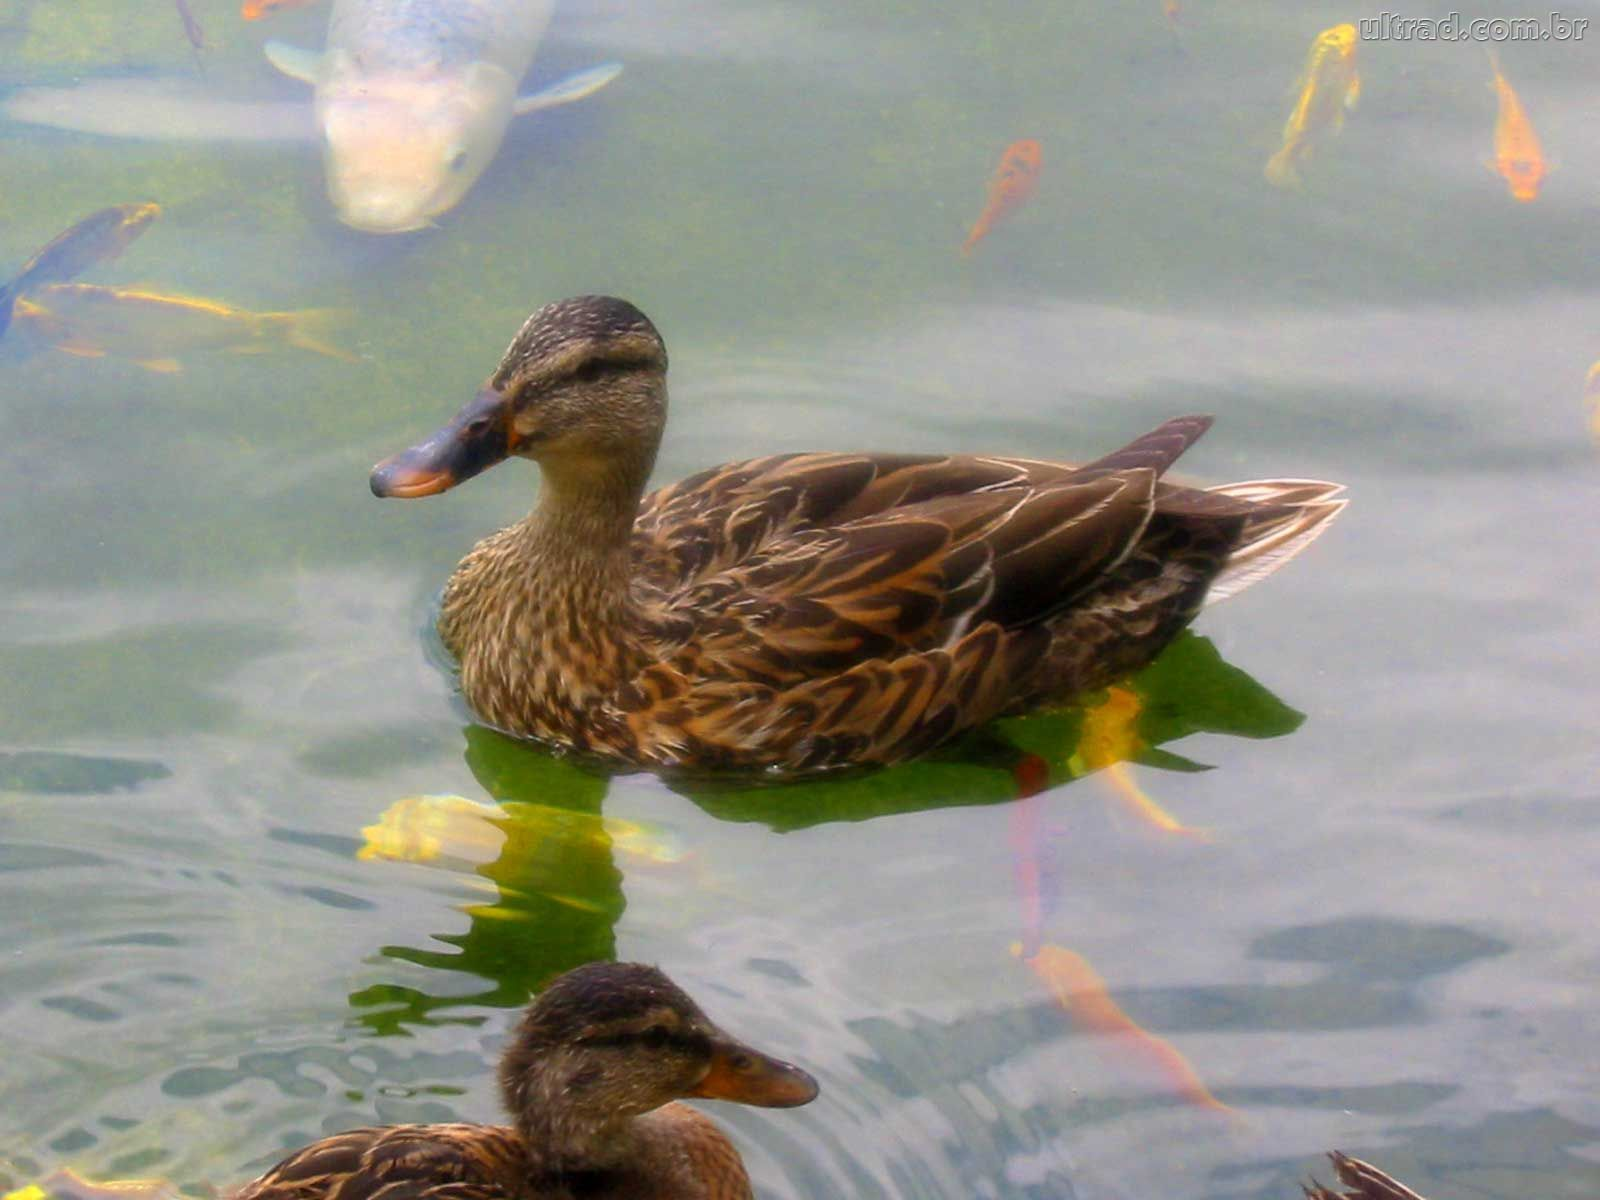
\includegraphics[scale=0.08]{./02-figuras/pato}
  \label{fig:patoA}
\end{center}

Artigos como mais de duas colunas não suportam o ambiente "figure" utilizado neste modelo \LaTeX. Uma alternativa para este problema é a inclusão do pacote:

{\tiny
\begin{verbatim}
    \usepackage{caption}
\end{verbatim}
}

e das seguintes linhas de comando:

{\tiny
\begin{verbatim}
    \begin{center}
      \captionof{figure}{<caption da figura>} 
      \includegraphics[<comandos alternativos>]
      		{<caminho ou nome da figura>}
      \label{<nome da referencia da figura>}
    \end{center}
\end{verbatim}
}



% -----------------------------------------------------------------------------
% Nova subseção
% -----------------------------------------------------------------------------

\subsection{Figura ocupando duas colunas} 		% edite para alterar o título da subseção

O ambiente \verb+figure+ pode ser usado em um artigo quando a figura for centralizada entre as margens do artigo (ocupa um espaço maior que uma coluna). Porém é necessário a introdução do \verb+*+ após o comando \verb+figure+.

\begin{figure*}
	\centering
	\caption{Pato na lagoa. Fator de escala: 20\% da original} 
	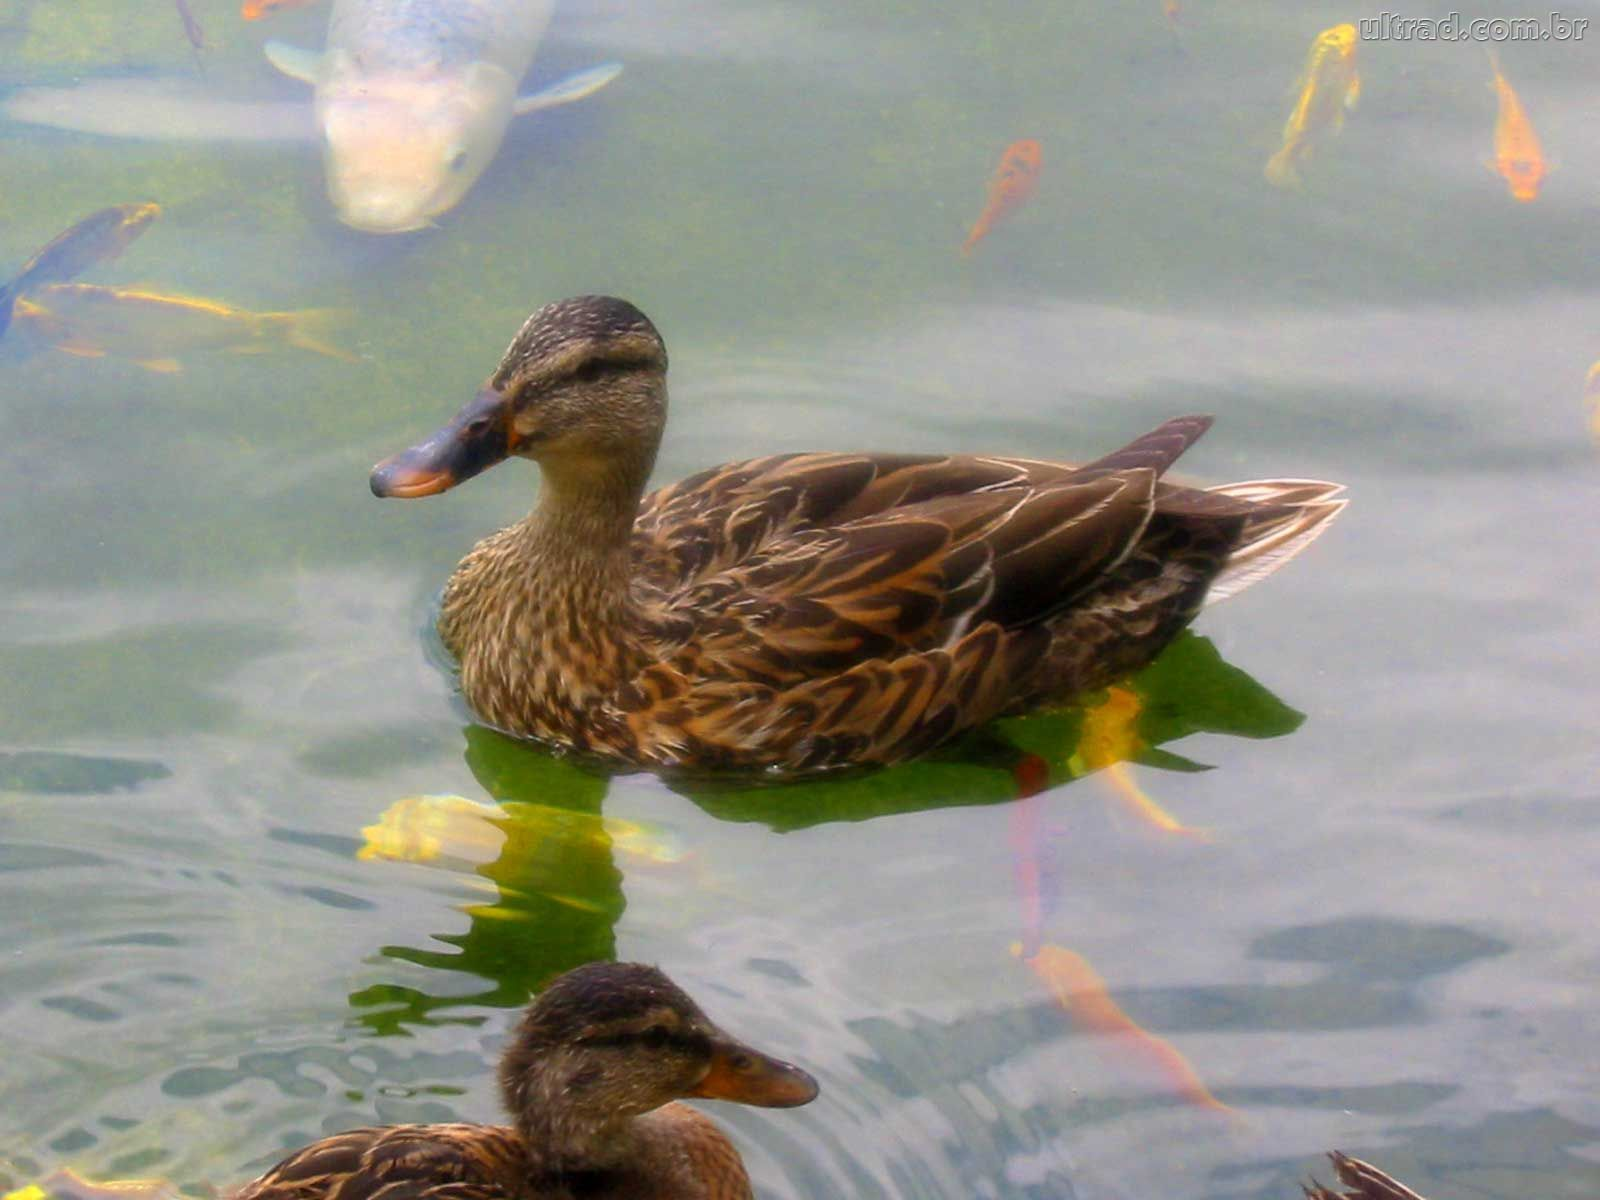
\includegraphics[scale=0.2]{./02-figuras/pato}
	\label{fig:patoB}
\end{figure*}

A \textbf{Figura \ref{fig:patoB}} foi inserida no artigo utilizando o comando \verb+figure*+ para o ambiente de figura.

{\tiny
\begin{verbatim}
   \begin{figure*}
     \centering
     \caption{Pato na lagoa. Fator de escala: 20\% da original} 
     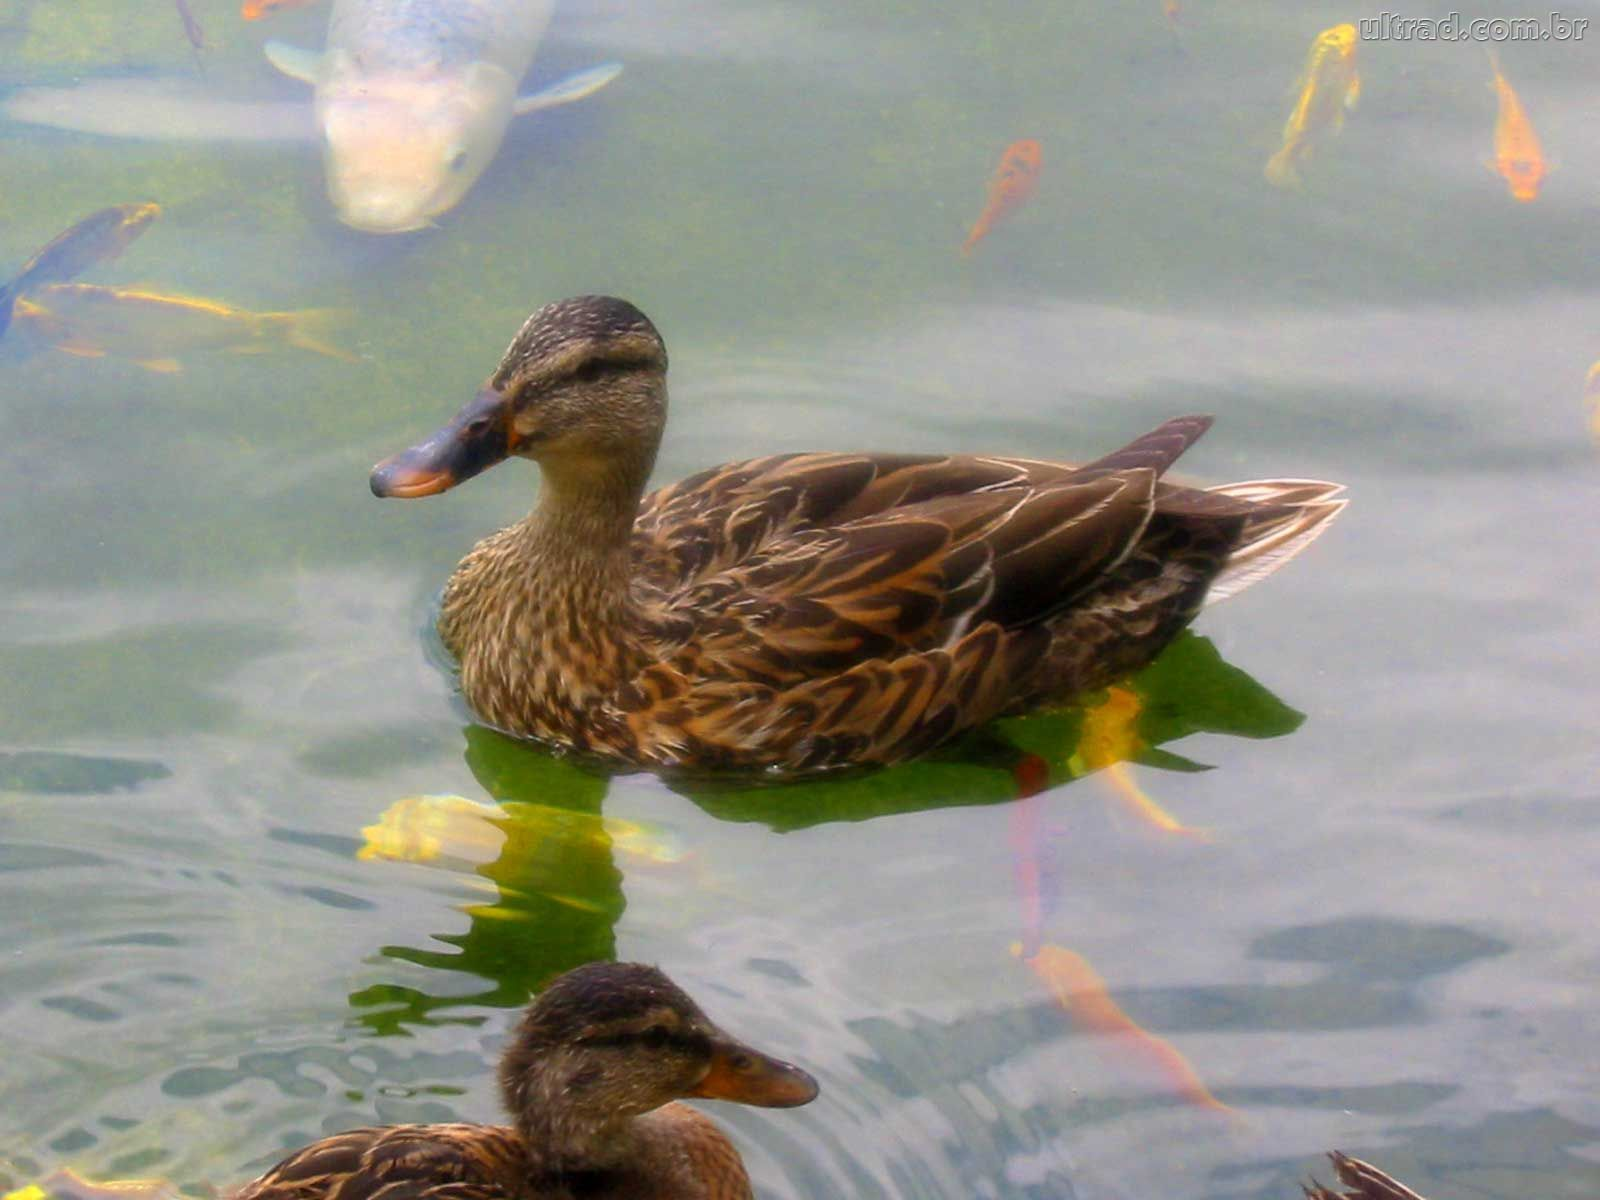
\includegraphics[scale=0.2]{./02-figuras/pato}
     \label{fig:patoB}
   \end{figure*}
\end{verbatim}
}



% -----------------------------------------------------------------------------
% Nova subseção
% -----------------------------------------------------------------------------

\subsection{Tabelas} 		% edite para alterar o título da subseção

O ambiente de tabelas é inserido no texto de modo análogo àquele feito no ambiente de figuras.




% -----------------------------------------------------------------------------
% Nova subseção
% -----------------------------------------------------------------------------

\subsection{Citações de referências} 		% edite para alterar o título da subseção

As referências são inseridas no texto como em qualquer documento em \LaTeX. Quando o nome do autor da referência faz parte do texto que você está escrevendo use o comando  \verb+\citeonline{}+ e quando este não for o caso use o comando \verb+\cite{}+. Veja a diferença entre os dois nas seguintes frases:

\noindent\textbf{(1)} Conforme discute \citeonline{kim1996} o resultado [...].

\noindent\textbf{(2)} Alternativamente a literatura\cite{kim1996} indica que o resultado [...].

Quando se tem mais de uma referência a ser citada em um mesmo certo trecho, há duas possibilidades de referenciá-las:

\noindent\textbf{(1)} colocar todas as referências em um único colchete (\emph{i.e.}, num mesmo comando \verb+\cite+),


\cite{kim1996,Wikibooks2009}

	
\noindent\textbf{(2)} colocar cada referência em seu próprio colchete (\emph{i.e.}, usando vários comandos \verb+\cite+ consecutivos),


\cite{kim1996}\cite{Wikibooks2009}

	% Arquivo a ser editado: contém a seção de “desenvolvimento” do artigo
% -----------------------------------------------------------------------------
%   Arquivo: ./01-texto/conclusao.tex
% -----------------------------------------------------------------------------


\section{Conclusão}\label{sec:conclusao}

Edite esta seção para colocar a conclusão de seu trabalho de pesquisa.

Procure fazer uma análise crítica de seu trabalho, destacando os principais resultados e as contribuições deste trabalho para a área de pesquisa.

Também deve indicar, se possível e/ou conveniente, como este trabalho pode ser estendido ou aprimorado.


		% Arquivo a ser editado: contém a seção de “conclusão” do artigo

	% Caso necessário, qualquer dos arquivos anteriores podem ser copiados e renomeados de modo a criar novas seções


%   Insere elementos pós-textuais

% -----------------------------------------------------------------------------
%   Arquivo: ./01-texto/agradecimentos.tex
% -----------------------------------------------------------------------------


\chapter{Agradecimentos}\label{sec:agradecimentos}
Edite e coloque aqui os agradecimentos às pessoas e/ou instituições que contribuíram para a realização do trabalho.

É obrigatório o agradecimento às instituições de fomento à pesquisa que financiaram total ou parcialmente o trabalho, inclusive no que diz respeito à concessão de bolsas.
	% Arquivo a ser editado: contém os “agradecimentos” a pessoas e/ou instituições que apoiaram a realização do trabalho
			% Não se pode esquecer de agradecer apropriadamente às instituições de fomento à pesquisa
% -----------------------------------------------------------------------------
%   Arquivo: ./01-texto/abstract.tex
% -----------------------------------------------------------------------------


\chapter{Abstract}\label{sec:abstract}
Translation of the abstract into english, possibly adapting or slightly changing the text in order to adjust it to the grammar of Standard English.




% -----------------------------------------------------------------------------
%   Edite o texto acima. Mantenha o limite de 200 palavras, bem como a formatação em parágrafo único.
% -----------------------------------------------------------------------------			% Arquivo a ser editado: contém o “abstract” em inglês
% -----------------------------------------------------------------------------
%   Arquivo: ./04-referencias/referencias.tex
% -----------------------------------------------------------------------------



% -----------------------------------------------------------------------------
%   Carrega o arquivo “myRefs.bib” e extrai automaticamente as referências citadas
% -----------------------------------------------------------------------------

\bibliography{./04-referencias/myRefs}{}
\bibliographystyle{abntex2-alf}		% Define o estilo ABNT para formatar a lista de referências  


% -----------------------------------------------------------------------------
%   Este arquivo não necessita de ser editado.
% -----------------------------------------------------------------------------	% Arquivo não-editável: carrega o arquivo “myrefs.bib” (coloque-o no diretório raiz) e o formata conforme a ABNT

\end{document}
